\documentclass[10pt]{article}
%Packages
\usepackage{multirow}
\usepackage{multicol}
\usepackage{color}
\usepackage{xcolor}
\usepackage{listings}
\usepackage{caption}
\usepackage{multicol}

%Math
\usepackage{amsmath}
\usepackage{amsfonts}
\usepackage{amssymb}
\usepackage{amsthm}
\usepackage{ulem}
\usepackage{stmaryrd} %f\UTF{00FC}r Blitz!


%PageStyle
\usepackage[ngerman]{babel} % deutsche Silbentrennung
\usepackage[utf8]{inputenc}
\usepackage{fancyhdr, graphicx}
\usepackage[scaled=0.92]{helvet}
\usepackage{enumitem}
\usepackage{parskip}
\usepackage[a4paper,top=2cm]{geometry}
\usepackage{graphicx}
\setlength{\textwidth}{17cm}
\setlength{\oddsidemargin}{-0.5cm}


% Shortcommands
\newcommand{\Bold}[1]{\textbf{#1}} %Boldface
\newcommand{\Kursiv}[1]{\textit{#1}} %Italic
\newcommand{\T}[1]{\text{#1}} %Textmode
\newcommand{\Nicht}[1]{\T{\sout{$ #1 $}}} %Streicht Shit durch

%Arrows
\newcommand{\lra}{\leftrightarrow}
\newcommand{\ra}{\rightarrow}
\newcommand{\la}{\leftarrow}
\newcommand{\lral}{\longleftrightarrow}
\newcommand{\ral}{\longrightarrow}
\newcommand{\lal}{\longleftarrow}
\newcommand{\Lra}{\Leftrightarrow}
\newcommand{\Ra}{\Rightarrow}
\newcommand{\La}{\Leftarrow}
\newcommand{\Lral}{\Longleftrightarrow}
\newcommand{\Ral}{\Longrightarrow}
\newcommand{\Lal}{\Longleftarrow}

% Java Code listenings
\DeclareCaptionFont{white}{\color{white}}
\DeclareCaptionFormat{listing}{\colorbox{gray}{\parbox{\textwidth}{#1#2#3}}}
\captionsetup[lstlisting]{format=listing,labelfont=white,textfont=white}

% XML Snippet Listings
\definecolor{gray}{rgb}{0.4,0.4,0.4}
\definecolor{darkblue}{rgb}{0.0,0.0,0.6}
\definecolor{cyan}{rgb}{0.0,0.6,0.6}

\lstset{
basicstyle=\ttfamily,
columns=fullflexible,
showstringspaces=false,
commentstyle=\color{gray}\upshape
}

\lstdefinestyle{JavaStyle}{
language=Java,
basicstyle=\footnotesize\ttfamily, % Standardschrift
numbers=left,               % Ort der Zeilennummern
numberstyle=\tiny,          % Stil der Zeilennummern
stepnumber=5,              % Abstand zwischen den Zeilennummern
numbersep=5pt,              % Abstand der Nummern zum Text
tabsize=2,                  % Groesse von Tabs
extendedchars=true,         %
breaklines=true,            % Zeilen werden Umgebrochen
frame=b,
%commentstyle=\itshape\color{LightLime}, Was isch das? O_o
%keywordstyle=\bfseries\color{DarkPurple}, und das O_o
basicstyle=\footnotesize\ttfamily,
stringstyle=\color[RGB]{42,0,255}\ttfamily, % Farbe der String
keywordstyle=\color[RGB]{127,0,85}\ttfamily, % Farbe der Keywords
commentstyle=\color[RGB]{63,127,95}\ttfamily, % Farbe des Kommentars
showspaces=false,           % Leerzeichen anzeigen ?
showtabs=false,             % Tabs anzeigen ?
xleftmargin=17pt,
framexleftmargin=17pt,
framexrightmargin=5pt,
framexbottommargin=4pt,
showstringspaces=false      % Leerzeichen in Strings anzeigen ?
}


\lstdefinelanguage{XML}
{
morestring=[b]",
morestring=[s]{>}{<},
morecomment=[s]{<?}{?>},
stringstyle=\color{black},
identifierstyle=\color{darkblue},
keywordstyle=\color{cyan},
morekeywords={xmlns,type}% list your attributes here
}


%Config
\renewcommand{\headrulewidth}{0pt}
\setlength{\headheight}{15.2pt}

%Metadata
\fancyfoot[C]{If you use this documentation for an exam, you should offer a beer to the authors!}
\title{
\vspace{2cm}
\textbf{Software Construction}
}
\author{Florian Thi\'event}
\date{3. Semester (HS 2018)}


% hier beginnt das Dokument
\begin{document}

    % Titelbild
    \maketitle
    \begin{center}
        \vspace{3cm}
        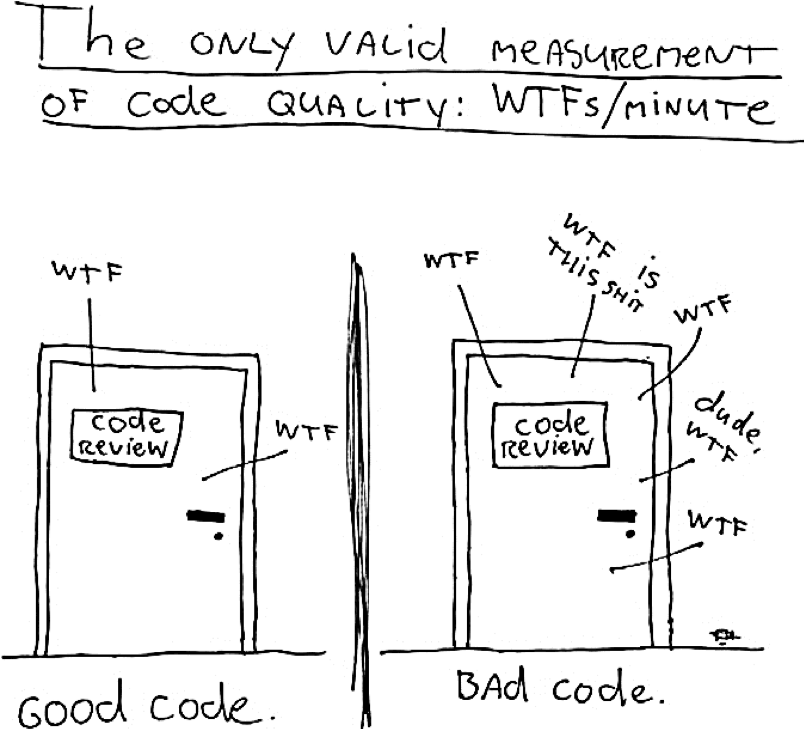
\includegraphics{assets/Titelbild.png}
        \thispagestyle{fancy}
    \end{center}
    \newpage

    % Inhaltsverzeichnis
    \pagenumbering{Roman}
    \tableofcontents
    \newpage
    \setcounter{page}{1}
    \pagenumbering{arabic}

    % Inhalt Start

    \section{Software Construction}
    \begin{tabular}{p{50mm} p{50mm} p{50mm}}
        \begin{center}
            Problem Definition \newline
            Anforderungen spezifizieren\newline
            \textbf{Planung der Anwendung}\newline
            SoftwareArchitektur\newline
        \end{center}
        &
        \begin{center}
            \textbf{\uline{Detail Plan}}\newline
            \textbf{\uline{Coding and Debugging}}\newline
            \textbf{\uline{Unit Testing}}\newline
        \end{center}
        &
        \begin{center}
            Team Management\newline
            Maintenance (Betrieb)\newline
            \textbf{Integration}\newline
            \textbf{Integration Testing}\newline
            System Testing\newline
        \end{center}
    \end{tabular}

    \subsection{Definition}
    Software construction is a fundamental act oft software engineering: the construction of working, \textbf{meaningful software} through a combination of \textbf{coding, validation and testing} by a programmer.
    \subsection{Low Level SWC}
    \begin{itemize}
        \item Testing definieren
        \item Design und Klassen schreiben
        \item Erstellen und Naming der Variablen und Konstanten
        \item Unit Testing, Integration Testing und Debugging
        \item Review von anderem Code von Teammitgliedern
        \item Integration von Software
        \item Formatierung von Code und Kommentaren
    \end{itemize}

    \subsection{Wieso ist SWC wichtig}
    \textbf{Construction is the only activity that's guaranteed to be done}
    \begin{center}
        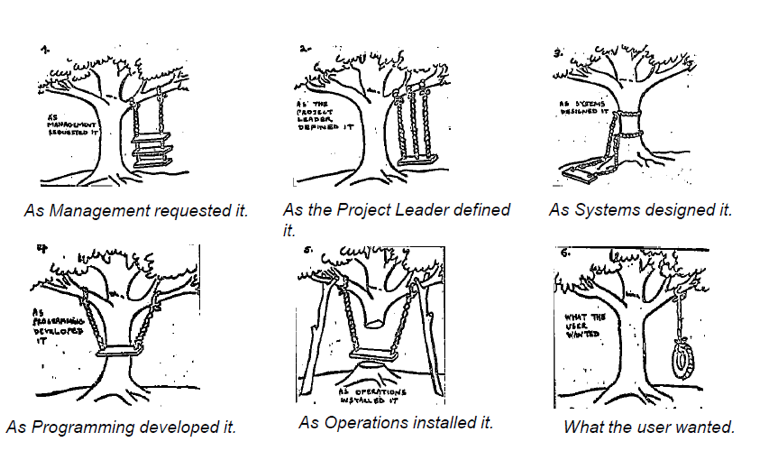
\includegraphics[width=0.8\textwidth]{assets/typical_project.png}
    \end{center}

    \subsection{Software Qualit\"at}
    \begin{itemize}
        \item Reliability: Zuverl\"assige Software welche fehlerfrei betrieben werden kann
        \item Reusability: Code Teile auch f\"ur andere Projekte nutzbar machen
        \item Extendibility: Erweiterbarkeit soll einfach m\"oglich sein
        \item Understandability: Code soll verst\"andlich f\"ur andere sein
        \item Efficiency: Geschwindigkeit
        \item Usability: Software einfach nutzen, auf das Zielpublikum ausgerichtet
        \item Portability: Einfach in eine andere Umgebung z\"ugeln
        \item Functionality: Software soll funktional sein
    \end{itemize}
    \textbf{Definition ISO:} The totality of features and characteristics of a product or service that bear on its ability stated or implied needs
    \\
    \textbf{Definition IEEE:} The degree to which a system, component, or process meets specified requirements.

    \subsection{Ziele}
    Die Software muss den Anforderungen des Kunden entsprechen. \textbf{"Good enough Software" not excellent software!}

    \subsection{Extreme Programming}
    \begin{enumerate}
        \item Der Kunde/Auftraggeber ist immer verf\"ugbar
        \item Code wird gem\"ass vereinbarten Standards programmiert
        \item Zuerst die Tests programmieren, dann den eigentlichen Code
        \item Der produktive Code wird immer zu zweit programmiert
        \item Nur ein Programmierer-Paar darf gleichzeitig Code integrieren
        \item Integriere h\"aufig
        \item Jeder hat auf den gesamten Code Zugriff
        \item Optimiere so sp\"at wie m\"oglich
        \item Keine \"uberstunden
        \item Das Team folgt gemeinsamen Code-Richtlinien, so dass es aussieht, als wenn der Code von einer einzigen Person geschrieben worden w\"are
        \item XP Projekte werden in sehr kurzen Abst\"anden released (von t\"aglich bis zu maximal alle 3-4 Wochen)
    \end{enumerate}
	%Neues Kapitel, neue Seite
	\newpage

    \section{Version Control System}
    Es geht grunds\"atzlich um sich st\"andig \"andernde Artefakte welche verwaltet werden m\"ussen. Jede \"anderung soll eindeutig nachvollziehbar sein.

    \subsection{Motivation f\"ur eine VCS}
    Ohne Versionsmanagement sieht der Alltag von Entwicklern so aus:
    \begin{itemize}
        \item Bugs die behoben wurden tauchen pl\"otzlich wieder auf
        \item Dateien gehen verloren
        \item Fr\"uhere Releases der Software k\"onnen nicht mehr erstellt werden
        \item Dateien werden "auf mysteri\"ose Art und Weise" ver\"andert
        \item Gleicher oder \"ahnlicher Code existiert mehrfach in verschiedenen Projekten
        \item Zwei Entwickler \"andern dieselbe Datei gleichzeitig ohne es zu merken
    \end{itemize}

    \subsection{Problem of Filesharing}
    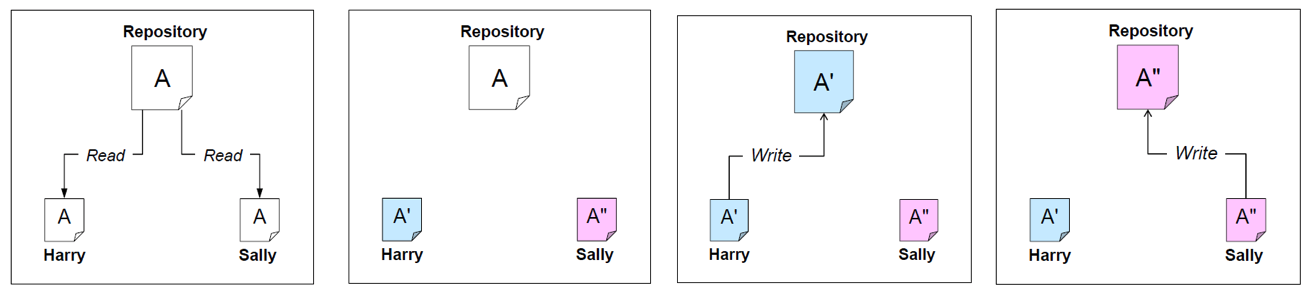
\includegraphics[width=0.9\textwidth]{assets/problem_of_filesharing.png}

    \subsection{Lock-Modify-Unlock Solution}
    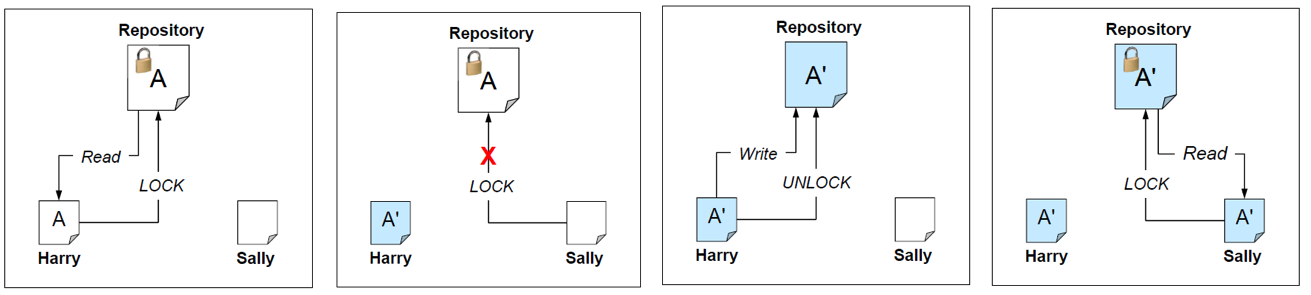
\includegraphics[width=0.9\textwidth]{assets/lock_modify_unlock_solution.png}

    \subsection{Copy-Modify-Merge Solution}
    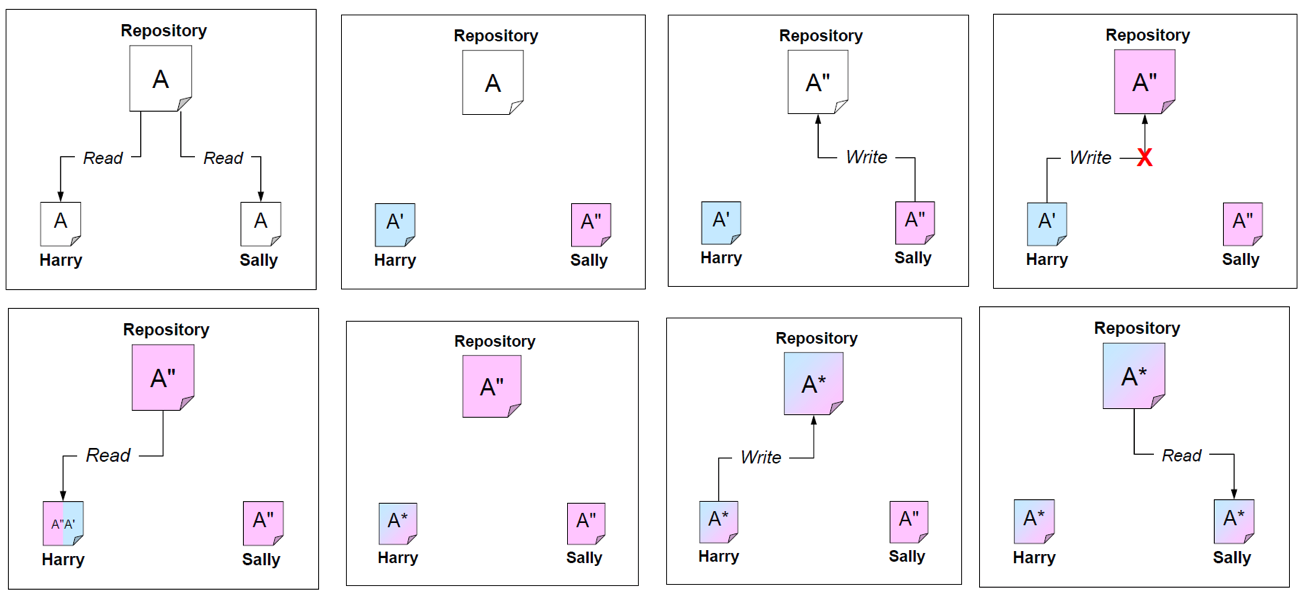
\includegraphics[width=0.9\textwidth]{assets/copy_modify_merge_solution.png}

    \subsection{Grundbegriffe Versions- und Release-Management}
    \subsubsection{Version}
    Ein Zustand eines Konfigurationselementes mit einem klar definierten Funktionsumfang.
    \subsubsection{Release}
    Bezeichnet eine ver\"offentlichte Version eines Konfigurationselementes. Oft wird ein Release auch ausserhalb der Software-Entwicklungsorganisation zusammengestellt.
    \subsubsection{Major}
    Die Idee, das Major-Versionen (mindestens teilweise) inkompatibel sind
    \subsubsection{Minor}
    \"anderungen dieser Nummer sind r\"uckw\"arts kompatibel.
    \subsubsection{Patch}
    Bug-Fixes, \"anderungen sind vorw\"arts- und r\"uckw\"arts kompatibel.
    \subsubsection{Build}
    Diese Nummer gibt eine Neukompilierung von Sourcecode an, z.B. aufgrund von Prozessor-, Plattform- oder Compiler\"anderungen.
    \subsubsection{Revision}
    Kleine \"anderung an einer Version, welche Fehler behebt, jedoch keine Einfluss auf den Funktionsumfang haben.
    \subsubsection{Variante}
    Eine Variation einer Version welche entwickelt wurde um z.B. auf einer anderen Hardware oder unter einem anderen Betriebssystem zu laufen. Oder auch um f\"ur verschiedene Benutzergruppen feine Anpassungen vorzunehmen. Beispiele: Anpassungen f\"ur Tablets, Sehbehinderte, Touchscreens.
    \subsection{Grundbegriffe VCS}
    \subsubsection{Repository}
    Eine Datenbank in welcher Projektdateien gespeichert werden. Ein Repository vergisst nichts, d.h. es ist nicht m\"oglich eine Datei zu \"uberschreiben. Vielmehr wir einfach eine neue Version der Datei gespeichert, die alte bleibt weiterhin im Repository und es kann auch weiterhin zugegriffen werden.
    \subsubsection{Working Copy}
    Eine \textit{lokale Kopie} aller relevanten Projektdateien. Der Entwickler arbeitet immer auf dieser lokalen Kopie. Es wird also \textit{nie} direkt auf den Dateien im Repository gearbeitet.
    \subsubsection{Checkout / Clone}
    Ist die Bezeichnung f\"ur einen Vorgang wenn eine Working Copy vom Repository bezogen wird. Dies ist eine reine Leseoperation auf dem Repository. Dabei wird auf der Entwicklermaschine eine neue Working Copy angelegt.
    \subsubsection{Commit / Push}
    Bezeichnet den Vorgang wenn eine Datei oder ein ganzes Set an Dateien (neu oder ge\"andert) \textit{mit einer Beschreibung} ins Repository gespeichert wird. Man spricht auch davon diese unter Versionskontrolle zu stellen. Dies ist eine Schreiboperation auf dem Repository die \textit{atomar} erfolgt, d.h. pro Commit werden entweder alle oder gar keine Dateien ins Repository gespeichert. Damit ist sichergestellt, das das Set an Dateien konsistent ins Repository gespeichert wird. Es ist nicht m\"oglich, dass durch zwei gleichzeitige Commits die Dateien durcheinandergebracht werden.
    \subsubsection{Update / Fetch / Pull}
    Bezeichnet den Vorgang wenn Dateien aus dem Repository mit der eigenen Working Copy abgeglichen werden. Indem andere Entwickler ihre Arbeit committen erh\"alt das Repository neue Versionen welche auf den Working Copies der anderen Entwickler noch nicht vorhanden sind. Der Abgleich findet auf der Working Copy statt, f\"ur das Repository ist ein Updatevorgang somit eine reine Leseoperation.
    \subsubsection{Revision, Version}
    Jeder Commit ver\"andert den Inhalt des Repositories und erzeugt somit eine neue Version oder Revision des Repositories die eindeutig identifizierbar sein muss. Dies ist notwendig um sp\"ater wieder auf einen bestimmten Stand der Arbeit zur\"uckzukehren zu k\"onnen. Manche Repositories verwenden mehrstellige Versionsnummern (z.B. CVS), andere nummerieren die Commits einfach durch (z.B. Subversion) oder vergeben einen Hash (z.B. Git) als Identifikation.
    \subsubsection{Entwicklungsverlauf (Baseline, Codeline, Line of Development}
    Dies sind Bezeichnungen f\"ur eine Menge von relevanten Projektdateien die zusammen geh\"oren und die miteinander weiterentwickelt werden. Eine Working Copy enth\"alt all diese Dateien einmal. Ein Entwicklungsverlauf bezeichnet aber die gesamte Historie dieser Dateien w\"ahrend des Entwicklungsverlaufes. D.h. er enth\"alt alle relevanten Projektdateien in allen Versionen f\"ur einen bestimmten Entwicklungsverlauf. Ein Entwicklungsverlauf ist eindeutig \"uber seinen Revisionsverlauf gekennzeichnet. Der Hauptentwicklungsverlauf wird in Subversion oder CVS auch einfach \textit{trunk} genannt und in Git heisst er \"ublicherweise \textit{master}.

    \subsubsection{Branch}
    So wird eine Verzweigung von Entwicklungsverl\"aufen genannt. Branches sind selber auch wieder Entwicklungsverl\"aufe. Sie enthalten selber eine eigene, von anderen Entwicklungsverl\"aufen unabh\"angigen Historie. Je nach Versionsverwaltungssystem werden Branches unterschiedlich eingesetzt. Ein m\"ogliches Szenario ist z.B. wenn die Entwicklung an einer Version 2 weiterl\"auft (Hauptentwicklungsverlauf) und gleichzeitig die alte Version 1.x noch weiter gewartet werde soll (Branch).

    \subsubsection{Merging}
    Bezeichnet den Vorgang zwei Entwicklungsverl\"aufe zu vereinen. Dazu m\"ussen Dateien in unterschiedlichen Versionen zusammengef\"uhrt werden. Dies ist in der Regel ein manueller Vorgang der nur bedingt automatisiert werden kann. Wie beim Branching wird auch das Merging unterschiedlich unterst\"utzt von den verschiedenen Versionskontrollsystemen.

    \subsubsection{Tag, Label}
    Identifiziert bzw. markiert eine bestimmte Revision eines Entwicklungsverlaufes oder Configuration Items und f\"ugt ihm noch zus\"atzliche Informationen hinzu (z.B. gibt ihm einen bestimmten Namen oder Bemerkung wie beispielsweise: \glqq Release f\"ur Demo anl\"asslich Veranstaltung xxx\grqq). Tags sind konzeptionell keine Entwicklungsverl\"aufe sondern nur eine Momentaufnahme (Snapshot) eines solchen.

    \subsection{Configuration Items}
    \begin{center}
        \begin{tabular}{|lll|c}
            \hline
            Unter VCS & Nicht im VCS & Grenzfall \\
            \hline
            Sourcen & Testprotokolle (generiert) & DB \\
            Dokumentation & Testreports (generiert) & Video \\
            Kommunikation & Pers\"onliche Konfig (IDE) & Audio \\
            Tests & Javadoc $\rightarrow$ html &  \\
            Geteilte Config & DIE & \\
            Video / Audiofiles (kleine) & Compilate &\\
            & (.exe, .class, .jar & \\
            & Files aus anderen Projekten & \\
            & (Libraries, Vorlagen) & \\

            \hline
        \end{tabular}
    \end{center}
	%Neues Kapitel, neue Seite
	\newpage

    \section{Build - Automation}
    Die Komponenten einer Software werden per Knopfdruck erstellt. Macht meist mehrer Dinge auf einmal (Code compilieren, Tests durchlaufen, Checkout, Kopie auf Server, E-Mail). Der Buildvorgang kann auch automatisch gestartet werden.
    \subsection{Wieso wird dies ben\"otigt, Probleme}
    \begin{itemize}
        \item Die Entwickler k\"onnen die Applikation nicht zuverl\"assig lokal erstellen
        \item Fehlen einer konsistenten Versionierung
        \item Unit Testing ist nicht konsistent
        \item Status des Build ist nicht bekannt
        \item Abh\"angigkeiten von Komponenten ist nicht bekannt
        \item Entwicklung ist nicht transparent
        \item Handarbeit ist fehleranf\"allig
        \item Wiederholende Arbeit ist langweilig
        \item Automation ist auch Dokumentation
    \end{itemize}

    \subsection{Build Prozess}
    \begin{center}
    	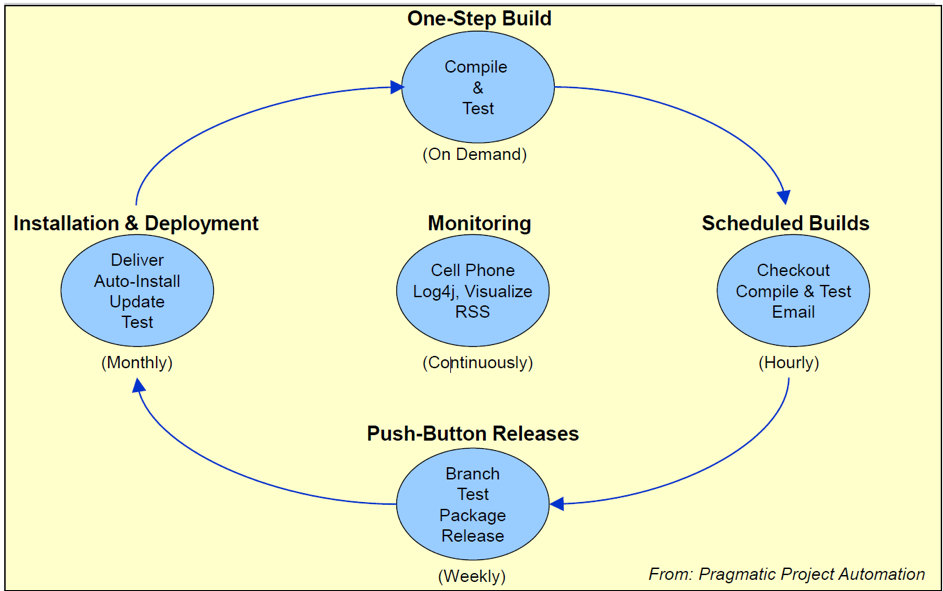
\includegraphics[scale=0.6]{assets/buildprozess.png}
    \end{center}
    
    \subsection{Ben\"otigte Komponenten}
    \begin{itemize}
        \item Build Server
        \item Source Code Control Server
        \item Prozesse
        \item Tools
        \item Entwickler Verantwortung (Code checked before end of day, buildable, passed unit test)
    \end{itemize}

    \subsection{CRISP}
    \begin{itemize}
        \item Complete (Tests erfolgreich, alle Komponenten enthalten)
        \item Repeatable (Wiederherstellung von alten Builds, keine Binary committen, bugfixing)
        \item Informative (Code Dokumentation, Infos f\"ur Merging)
        \item Schedulable (planbar, f\"ur Akronym)
        \item Portable (definierte Portabilit\"at, auch auf anderen System funktional)
    \end{itemize}

    \subsection{Maven}
    Maven ist ein Build Automation Tool und der de-facto Standard in Java Projekten. Maven setzt auf deklarative Konfiguration und folgten dem Ansatz Konvention vor Konfiguration. \textbf{Put the source in the correct directory and Maven will take care of the rest}.

    \subsubsection{Project Model (POM)}
    Enth\"alt die Informationen f\"ur den Output.
    
    \begin{multicols}{2}
    	\lstinputlisting[language=XML]{assets/minimal_pom.xml} 
    	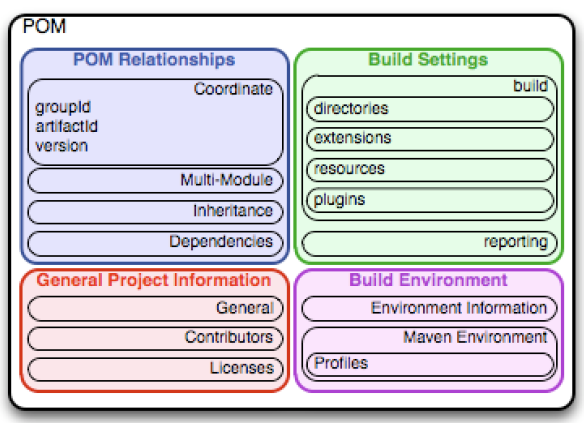
\includegraphics[scale=0.5]{assets/pom.png} \\
    \end{multicols}
    \begin{center}
    	   		\textbf{Pflichtfelder: groupeId, artifactId, version und packaging}
    \end{center}

    \subsubsection{Standard Build Prozess}
    \begin{center}
    	
    \begin{tabular}{|ll|c}
        \hline
        Begriff & Beschreibung  \\
        \hline
        \textbf{validate} & check if project is valid and all necessary information is available \\
        \textbf{process-resources} & convert and filter resource files \\
        \textbf{compile} & compile source code \\
        \textbf{test-compile} & compile test code \\
        \textbf{test} & Execute tests \\
        \textbf{package} & package the artifact \\
        \textbf{integration-test} & execute integration tests \\
        \textbf{install} & copy artifact into the local repository \\
        \textbf{deploy} & publish artifact in the remote repository \\
        \hline
    \end{tabular}
     \end{center}

    \subsubsection{Directory Structure}

			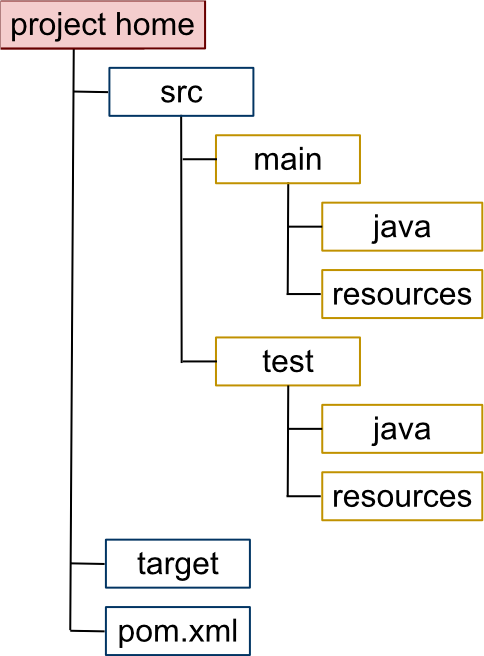
\includegraphics[scale=0.5]{assets/mvn_directory_structure}
               
                \begin{itemize}
                \item Java-Source (to be delivered)
                \item Non-Source Files (properties, icons \ldots)
                \item Test Classes
                \item Resources files
            \end{itemize}

	\newpage
    \subsubsection{Fallbeispiel POM}
    \lstinputlisting[language=XML]{assets/pom.xml}
	%Neues Kapitel, neue Seite
	\newpage
	

    \section{Clean Code}
    Clean code is \textbf{simple} and direct. Clean code reads like well-written prose. Clean code never obscures the designer\textquoteright s intent but rather is full of \textbf{crisp} abstractions and \textbf{straightforward} lines of control.

    \subsection{Grunds\"atze}
    \begin{itemize}
        \item Name der Variabel, Methode oder Klasse sollte den Zweck beinhalten.
        \item Variabeln sollten m\"oglichst nahe zum Aufrufpunkt deklariert werden
        \item Callers (Aufrufen) sollten oberhalb der Callees (Aufgerufene) deklaiert sein
        \item Lines short (80 Characters)
        \item Define Tabs vs. Spaces and Line Wrapping/Breaking Rules
        \item Use the Code Convention of the Programming Language
        \item Checkstyle integrieren
        \item Class Documentation (performance, memory consumption, persistence)
        \item Interface Doc (Explain what is done)
        \item Method Doc (precondition, postcondition, invariant) => bei Kommentaren Subjekt auslassen
        \item Use Javadoc
        \item Funktionen sollten nur eine Sache Machen
        \item Negative Konditionen sollten verhindert warden
    \end{itemize}

    \subsection{Wieso CleanCode}
    \begin{itemize}
        \item 80\% of the lifetime cost of a piece of software goes to maintenance.
        \item Code is written once, but read all other times
        \item Hardly any software is maintained for its whole life by the original author.
        \item Clean code improves the readability of the software, allowing engineers to understand new code more quickly and thoroughly.
    \end{itemize}

    \subsection{Konzepte}
    \subsubsection{Vertical Openness}
    Uses more vertical space (new line, brackets, etc) this improves readability, quick to see which code parts are not together.

    \subsubsection{Vertical density}
    Opennness separates concepts. Density implies association. Results in Compact Code.

    \subsubsection{Vertical Distance and Ordering}
    Concepts that are closely related should be vertically close to each other.
    \begin{itemize}
        \item Variables should be declared as close to their usage as possible.
        \item Instance variables should be declared at the top of the class.
        \item Dependent functions: callers should be above callees.
    \end{itemize}


    \subsubsection{Horizontal Openness and Density}
    \begin{itemize}
        \item Keep lines short.
        \subitem complete line should be displayable without scrolling (eg <120 characters per line)
        \item Don\textquoteright t try to horizontally align lists of assignments
        \subitem It draws attention to the wrong thing and can be misleading, e.g., encouraging the reader to read down a column.
        \item Always indent scopes (classes, methods, blocks).
        \item Avoid using tabs, replace them with spaces
        \item Define line wrapping, line breaking rules, e.g.:
        \subitem After comma
        \subitem Before operator, i.e. operators come first on new line
        \item Define clear spacing rules, e.g.
        \subitem Put spaces around = to accentuate the distinction between the LHS and RHS.
        \subitem Don\textquoteright t put spaces between method names and parenthesis, or parenthesis and parameter lists - they\textquoteright re closely related, so should be close.
        \subitem Use spaces to accentuate operator precedence, e.g., no space between unary operators and their operands, space between binary operators and their operands.
    \end{itemize}

    \subsubsection{Team Rules}
    \begin{itemize}
        \item Every team should agree on a coding standard
        \item Beware of code formatting standards getting religious.
        \item If the language you\textquoteright re using has a code convention (like Java\textquoteright s), use it!
    \end{itemize}
    %Neues Kapitel, neue Seite
	\newpage
	

    \section{Continous Integration}
    Integration ist verschiedene Module zusammen zum Laufen zu kriegen. Die Module m\"ussen zusammen kompiliert, gestartet, getestet und deployed werden k\"onnen. \textbf{CI reduziert Risiken und deckt Fehler fr\"uh auf.}

    \subsubsection{Fehlerhafte Integration}
    \begin{itemize}
        \item Integration Server kann den Build nicht durchf\"uhren
        \item Geteilte Inhalte funktionieren nicht in allen System
        \item Fehler bei Unit Tests
        \item Code Qualit\"at failed
        \item Deployment failed
    \end{itemize}

    \subsubsection{Arbeiten mit Continous Integration}
    \begin{itemize}
        \item Nur ein Source Repository
        \item Automatisierter Build
        \item Build testet sich selbst
        \item Jeder commited jeden Tag
        \item Der Build sollte schnell gehalten werden
        \item Testen auf einem Klone der Produktion
        \item Einfach das letzte executable zu erhalten
        \item Jeder sieht was sich \"andert
        \item Automatisiertes Deployment
    \end{itemize}
    \begin{center}
    	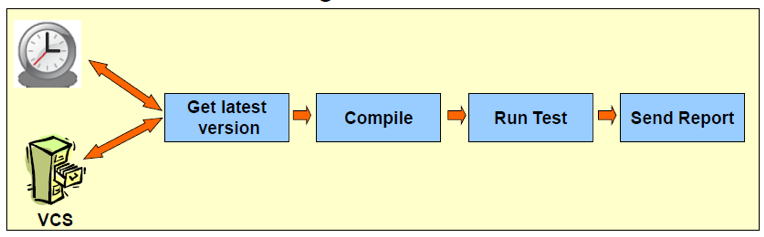
\includegraphics[scale=0.6]{assets/arbeit_ci.png}
	\end{center}


    \subsection{Prerequisites of Continuous Integration} 
    \begin{multicols}{2}
    	    \begin{itemize}
        \item VCS Server
        \item Build Server
        \item Deployment Server
        \item Automation tools
        \item CI tools
    \end{itemize}
    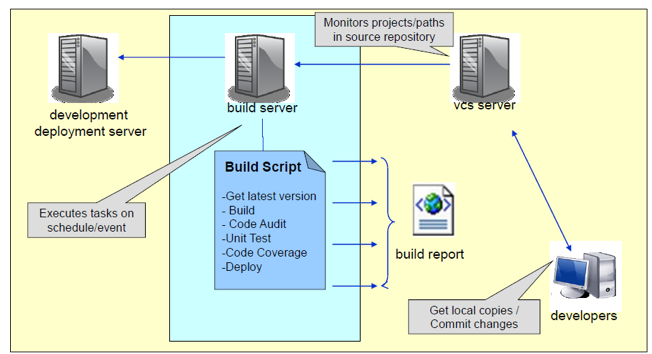
\includegraphics[scale=0.5]{assets/vorbedingung_ci.png}
    \end{multicols}   
	
	
    \subsection{Jenkins}
    Jenkins ist ein CI Server welcher building, unit tests, code coverage und weitere Punkte zur Verf\"ugung stellt.
    Gibt sofort einen Status \"uber den Build zur\"uck und hat ein Dashboard f\"ur die Integration von verschiedenen Projekten.

    \subsection{Jenkins Componenten und Add Ons}
    \begin{center}
        \begin{tabular}{|ll|}
            \hline
            Components & Add Ons \\
            \hline
            CI Server (Monitors the VCS and Execute Build Script) & Unit Testing \\
            Management Console & Test Code Coverage \\
            Dashboard & Analysis \\
            Email Notification & Ant \\
            & Google Calender, and, and, and \\
            \hline
        \end{tabular}
    \end{center}
	%Neues Kapitel, neue Seite
	\newpage
	
	

    \section{Unit Testing}
    Testing von Softare ist extrem wichtig. Zum einen k\"onnen Fehler aufgedeckt und korrigiert werden. Somit k\"onnen Kosten eingespart werden. Falls es um Spezialsoftware geht k\"onnen sogar Menschenleben oder Umweltkatastrophen entstehen bzw. verhindert werden.
    \begin{itemize}
        \item Validation: Did you build the right thing?
        \item Verification: Did you build it right?
    \end{itemize}

    \subsection{Fault, Error and Failure}
    \subsubsection{Fault}
    A static defect in the software = the actual mistake or bug in the code.
    \subsubsection{Software Error}
    An incorrect internal state that is the manifestation of some fault.
    \subsubsection{Software Failure}
    External incorrect behavior with respect to the requirements or other description of the expected behavior.
    \subsection{Ablauf}
    \begin{itemize}
        \item Wird auf jede unit (Klasse, manchmal Methoden) durchgef\"uhrt
        \item In isolation
        \item Unit Test baut eine eigene Testumgebung auf
        \item Checkt das Resultat mit den erwarten Werten
        \item Test Spezifizierung
        \item Test Implementierung
        \item Setup und Cleanup definieren
    \end{itemize}


    \subsection{Schlechte Ausreden gegen Unit Testing}
    \begin{itemize}
        \item It takes too much time to write the tests
        \item It takes too long to run the tests
        \item It's not my job to test my codeI
        \item don't really know how the code is supposed to behave so I can't test it
        \item But it compiles
        \item I'm being paid to write code, not to write tests
        \item I feel guilty about putting testers and QA staff out of work
        \item My company won't let me run unit tests on the live system
    \end{itemize}

    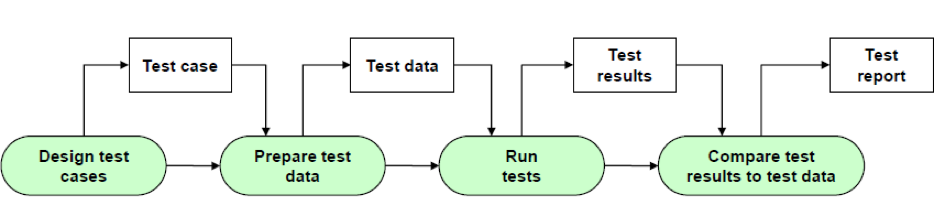
\includegraphics{assets/ablauf_unittesting.png}

    \subsection{JUnit}
    Standard in Java
    \subsubsection{Gute JUnit Tests}
    \begin{itemize}
        \item Automatic (Invoking the tests and checking the results)
        \item Thorough (test everything that is likely to break)
        \item Repeatable (ablte to run over and over again)
        \item Independant (no test relies on another test)
        \item Professional (use same standard as for production code)
        \item Do not test compiler, setters/getters
    \end{itemize}

    \subsubsection{Equivalent Klassen}
    Die Eingabewerte von Tests m\"ussen in verschiedene Equivalent Klassen eingegrenzt werden. In diesen Klassen soll der Grenzwert erkannt werden und zudem auch um die Grenzwerte getestet werden (off-by-one-errors)
    \subsubsection{Right BICEP}
    \begin{itemize}
        \item Right \textendash Sind die Resultate korrekt
        \item B \textendash Sind alle boundary (Grenzwerte) korrekt
        \item I \textendash K\"onnen auch Inverse Beziehungen getestet werden
        \item C \textendash Cross check
        \item E \textendash K\"onnen Errors erzwungen werden
        \item P \textendash Performance sind wie erwartet (was passiert wenn Input verdoppelt, verdreifacht wird)
    \end{itemize}

    \subsubsection{Grundbegriffe}
    \begin{itemize}
        \item Class under Test (CUT)
        \item Method under Test (MUT)
        \item Test Case (Spezifische daten welche f\"ur Test ausgew\"ahlt wurden @Before, @After,@Test)
        \item Test Suite (ein Set von verschiedenen Test Cases)
        \item Test Fixture (Die ganze Test Klasse)
    \end{itemize}

    \subsection{Testing in Isolation}
    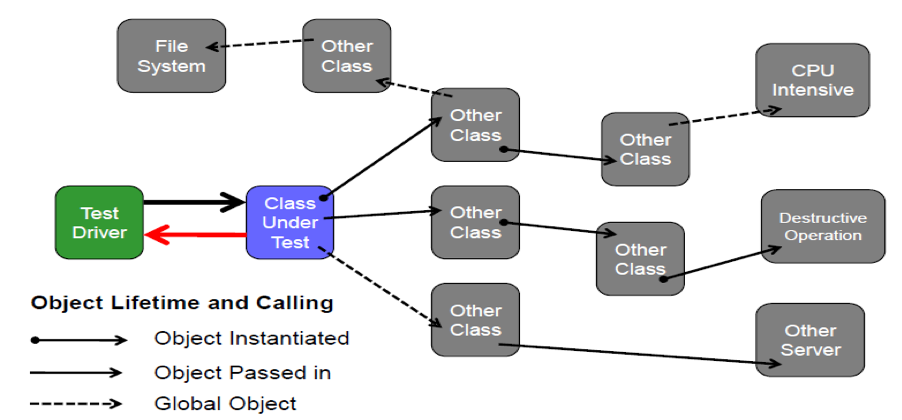
\includegraphics{assets/isolation_testing.png}
   
	Some things are difficult to test in isolation 
	\begin{itemize}
		\item Configuration
		\item Database Access
		\item Network Access
	\end{itemize}
	In general: How to test a class that depends on other components?
	
	\subsubsection{Test Doubles}
	A \textit{Test Double} is any object or component that is installed in place of the real component for the express purpose of running a test.
	
	\subsubsection{Test Doubles in Unit Testing}
	\begin{itemize}
		\item \textbf{Dummy objects} are passed around but never actually used. Usually they are just used to fill parameter lists.
		\item \textbf{Stubs} are minimal implementations of interfaces or base classes. Methods returning void will typically contain no implementation at all, while methods returning values will typically return hard-coded values.
		\item \textbf{Spies} similar to a stub, but a spy will also record which members were invoked so that unit tests can verify that members were invoked as expected.
		\item \textbf{Fakes} contain more complex implementations, typically handling interactions between different members of the type it\textquoteright s inheriting.
		\item \textbf{Mocks objects} pre-programmed with expectations about the methods that will be invoked. The expected arguments for a call and the resulting return values or exceptions
	\end{itemize}
    
    \subsubsection{Test Doubles - Stubs}
    \begin{itemize}
    	\item Stub is a dumb object!
		\item A Stub is just an object that returns the same value over and over again.
		\item Allows implementation of tests without production code.
    \end{itemize}
    \newpage
    For example: \begin{verbatim}
			class EmailStub implements EmailService{
  				void sendMail(String adr; String Text) {;}
			}
		\end{verbatim}
    
    \subsubsection{Stubs - Sample Application}
    \begin{center}
    	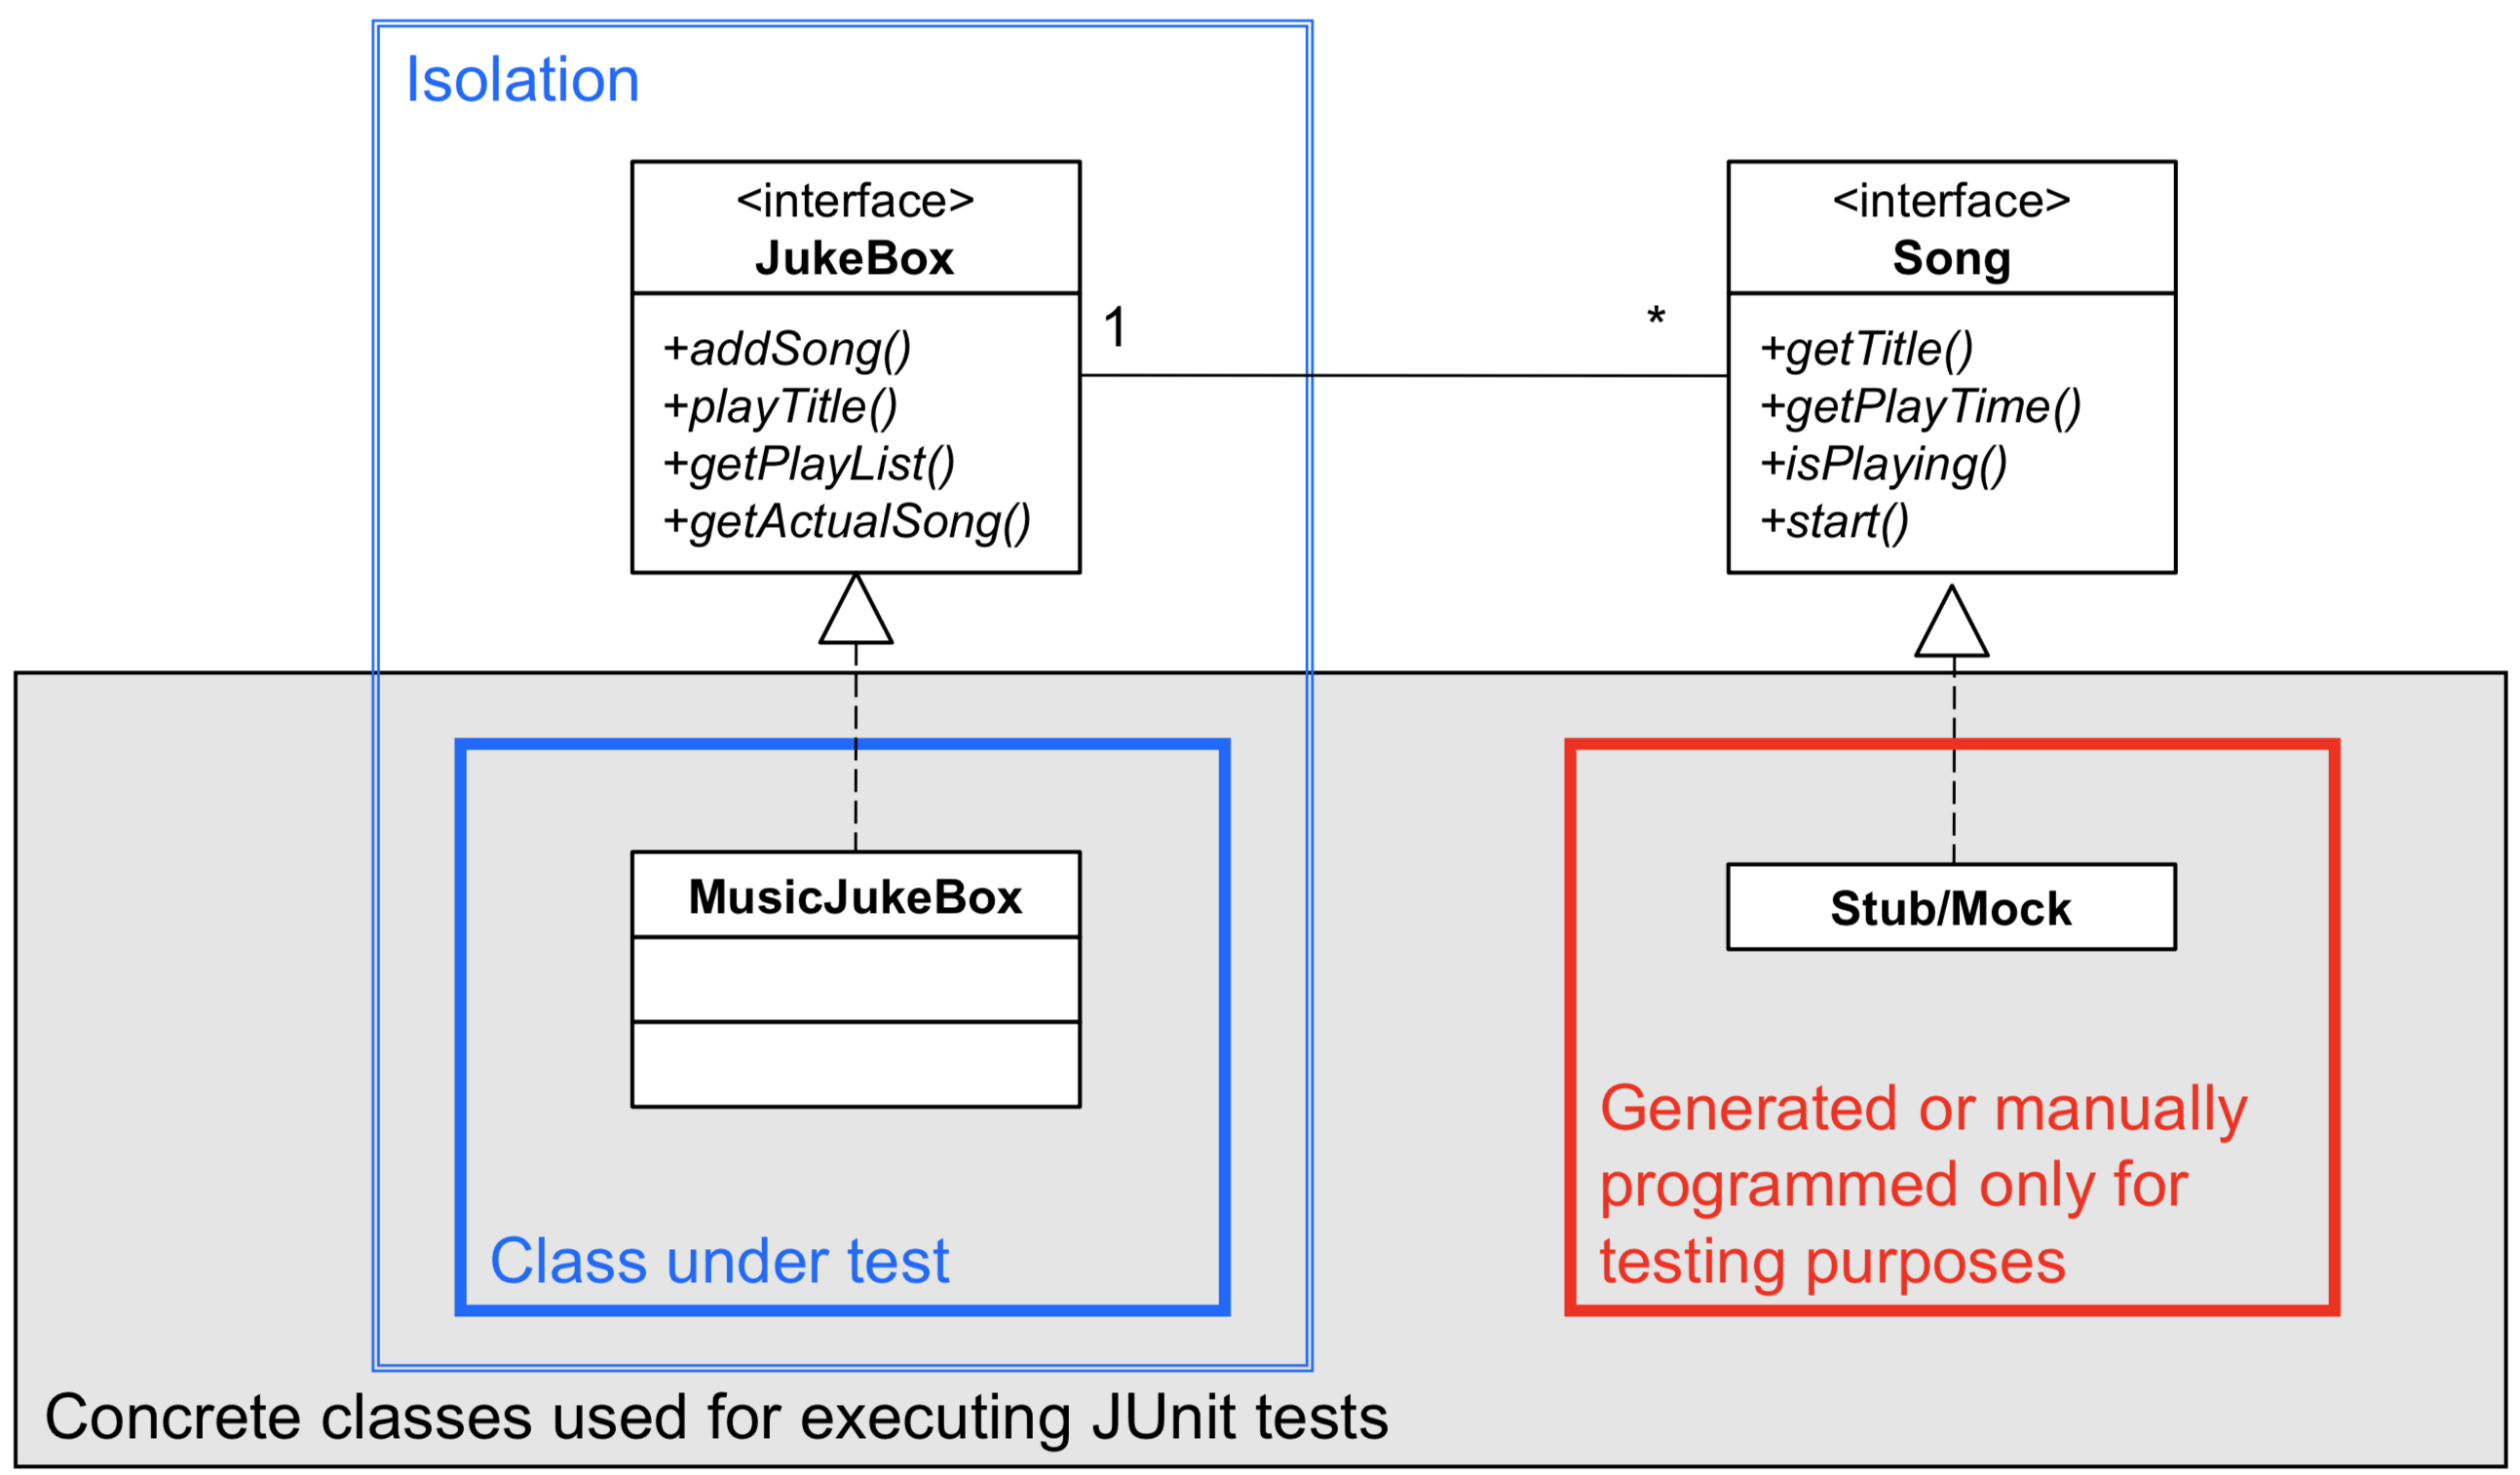
\includegraphics[scale=0.3]{assets/stubs.png}
    \end{center}
       
    \subsection{Mock Testing}
	%Neues Kapitel, neue Seite
	\newpage
	
	
	
	
    \section{Javadoc}
    \begin{itemize}
        \item Is a separate program that comes with the JDK
        \item Reads your program, makes lists of all the classes, interfaces, methods, and variables, and creates HTML pages displaying its results
        \item Its output is very professional looking
    \end{itemize}

    This makes \texttt{you} look good ... and it also helps keep your manager from imposing bizarre documentation standards
    \begin{itemize}
        \item Write comments for the programmer who uses your classes
    \end{itemize}
    Anything you want to make available outside the class should be documented. It is a good idea to describe, for your own use, private elements as wel. \texttt{javadoc} can be set to generate documentation for: only public elements
    \begin{itemize}
        \item public and protected elements
        \item public, protected, and package elements
        \item everything--that is, public, protected, package, and
        \item private elements
    \end{itemize}

    \subsection{Tags In javadoc Comments}
    Use the standard ordering for javadoc tags
    In method descriptions, use:
    \begin{verbatim}
        @param p A description of parameter p.
        @return A description of the value returned (unless the method returns void).
        @exception e Describe any thrown exception.
        @see Adds a "See Also" heading with a link or text entry that points to reference
    \end{verbatim}
    Don\textquoteright t use tags unless you maintain them!

    \subsection{Know Where To Put Comments!}
    javadoc comments must be immediately before: a package (only in package-info.java)
    \begin{itemize}
        \item a class
        \item an interface
        \item a constructor a method
        \item a field
    \end{itemize}
    Anywhere else, javadoc comments will be \textit{ignored}!

    \subsection{Hints}
    \begin{itemize}
        \item Keep comments up to date
        \item Use the word \grqq this \grqq rather than \grqq the \grqq when referring to instances of the current class.
        \item Hence, \texttt{this object} has an especially clear meaning in comments Example: \texttt{Decides which direction this frog should move.}(As a comment in the \texttt{Frog} class)
        \item Summarize the essence of your method, field or package comment in the first sentence.
        \item Javadoc copies the first sentence into a summary paragraph.
        \item Include examples if they are helpful.
    \end{itemize}
	%Neues Kapitel, neue Seite
	\newpage
	
	
	\section{Software Smells \& Refactoring }
	%Neues Kapitel, neue Seite
	\newpage
	
	\section{Metrics}
	Top 5 reasons why IT projects fail:
	\begin{enumerate}
		\item Communication problems
		\item Bad planning / lack of planning
		\item Lack of ressources
		\item Requirements and goals are not clear
		\item Politics
	\end{enumerate}
	So code quality isn’t an issue here?
	\subsection{Software Quality}
	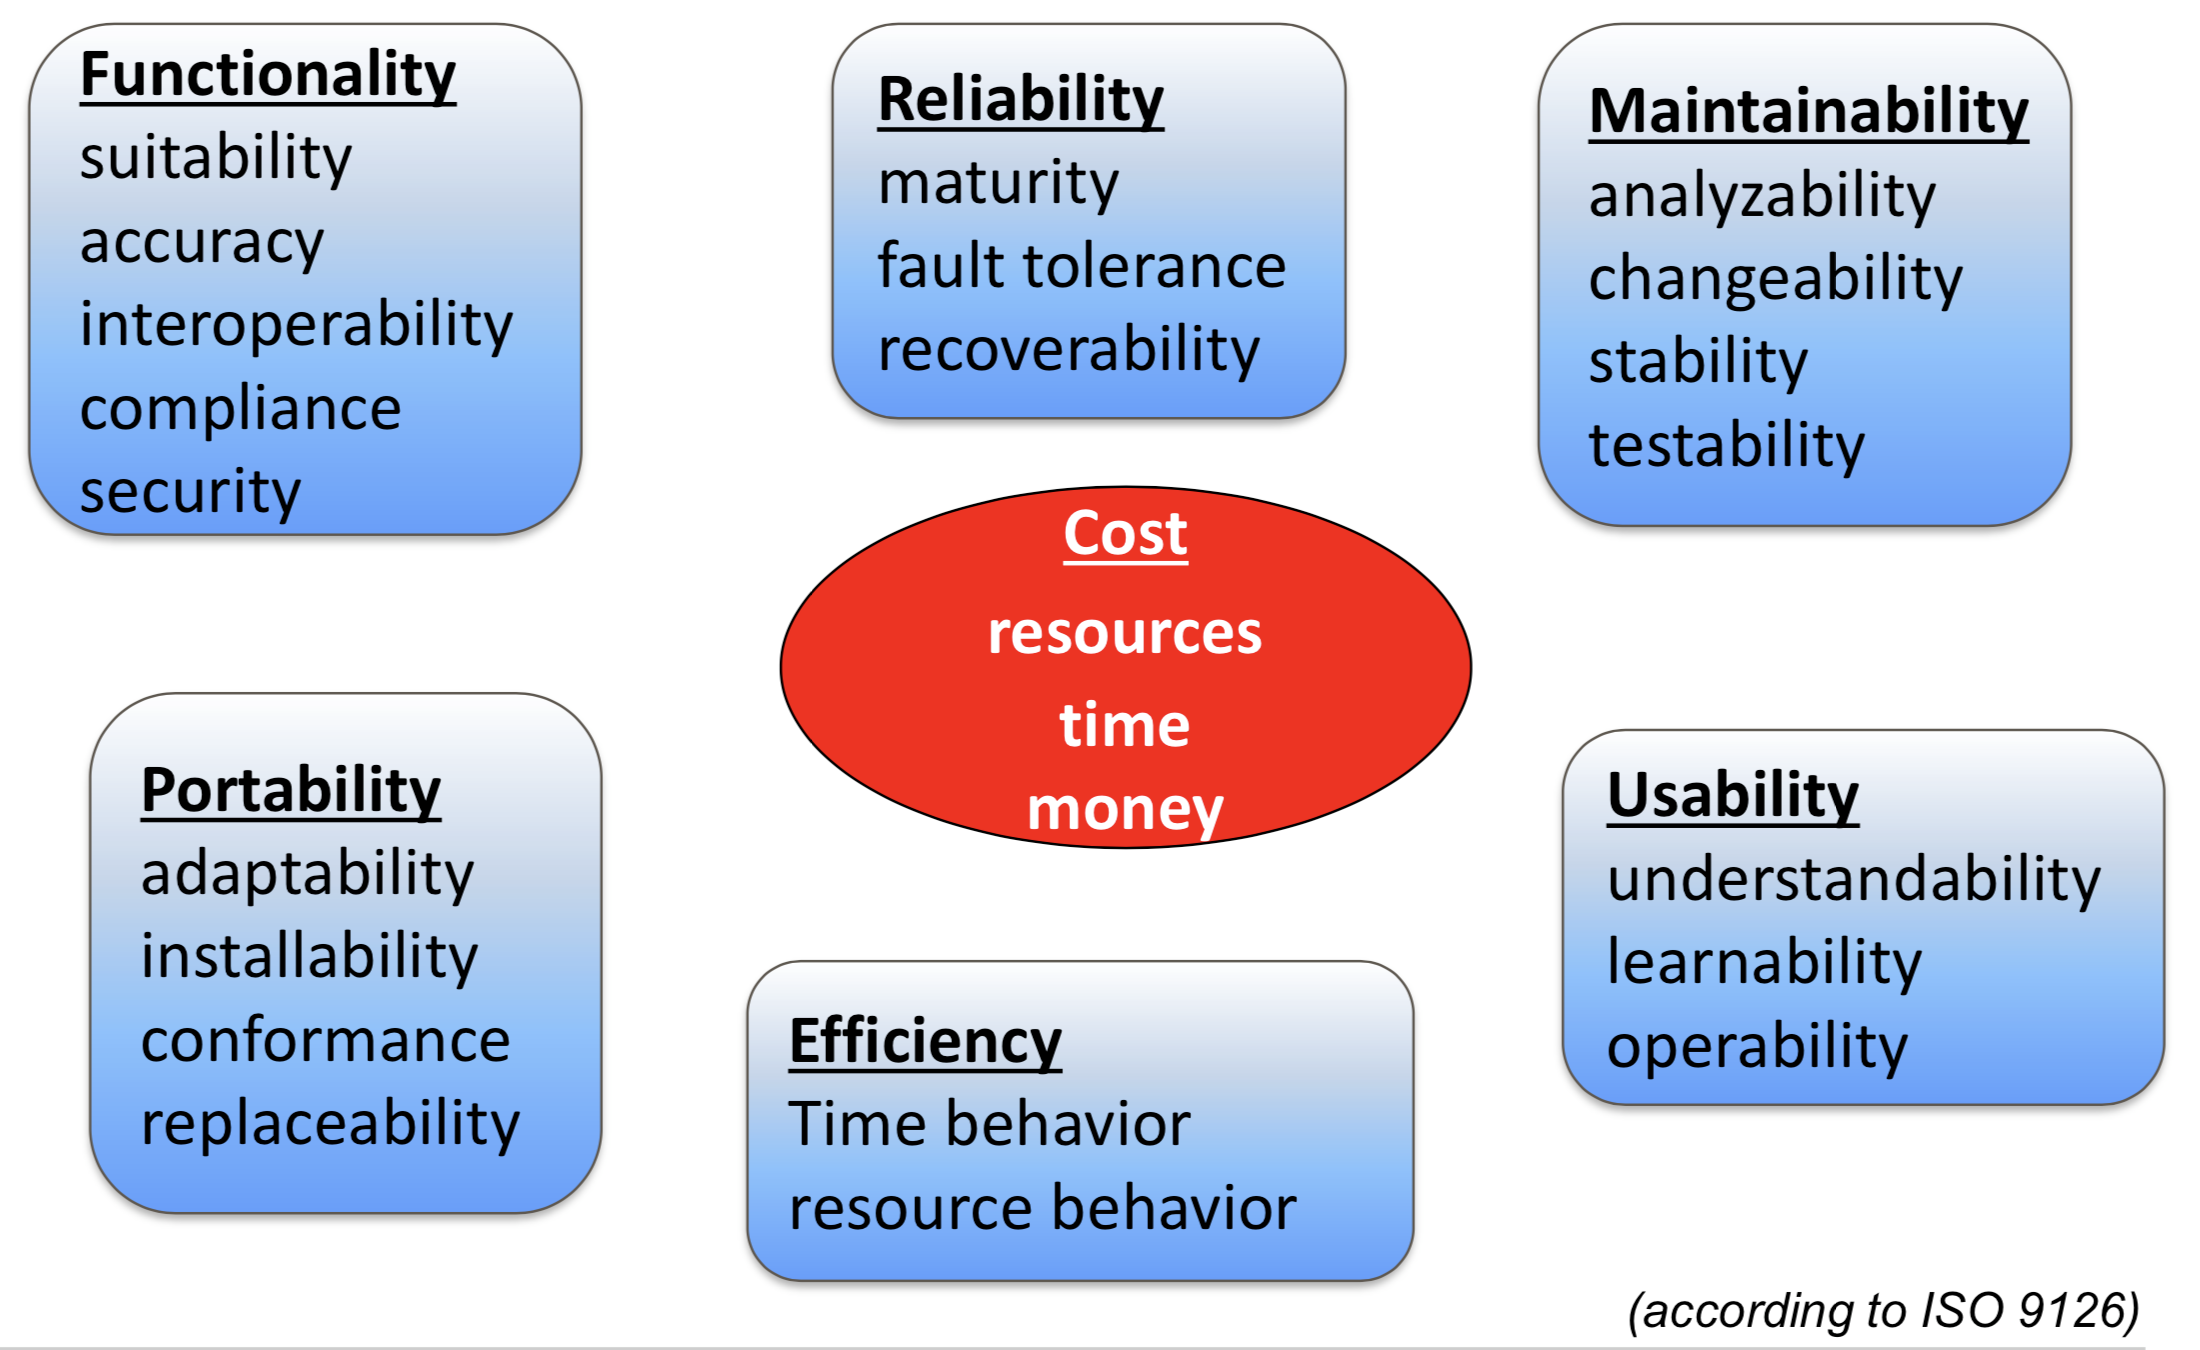
\includegraphics[scale=0.4]{assets/software_quality}
	
	\subsection{Characteristics of useful Metrics}
	A useful metric has four characteristics
	\begin{itemize}
		\item \textbf{Measurable:} If you can’t measure it, you can’t use it!
		\item \textbf{Independent:} A metric must be independent of any influence of the project members!→If they can manipulate the metric, it gets useless!
		\item \textbf{Reliable:} Conclusions drawn from metrics must be plausible. Therefore the raw data must be reliable.
		\item \textbf{Accurate:} Metrics must be accurate, to be useful. Even if the precision varies!
	\end{itemize}
	\subsection{Static Software Metrics}
	\begin{itemize}
		\item  Size Metrics
			\subitem Lines of Code; Number of Statements, Fields, Methods, Packages
		\item Dataflow Metrics
			\subitem Cyclomatic Complexity (McCabe Complexity)
    		\subitem Dead Code detection Initialization before use
			\subitem In Java: done by the compiler!
  		\item Style Metrics
			\subitem Number of Levels (nesting depth)
			\subitem Naming conventions, formatting conventions
		\item OO Metrics
			\subitem No. of classes, packages, methods Inheritance depth / width
		\item Coupling Metrics
			\subitem LCOM: lack of cohesion metrics
			\subitem No. of calling classes / no. of called classes Efferent / Afferent couplings
		\item Statistic Metrics 
			\subitem Instability
			\subitem Abstractness
	\end{itemize}
	
	\subsection{Dynamic Software Metrics}
	\begin{itemize}
		\item Performance Metrics Time spent
			\subitem Memory consumption (also memory leaks) 
			\subitem Network traffic
			\subitem Bandwidth needed
			\subitem No. of clicks to perform a task
		\item Other Dynamic Metrics
			\subitem No. of tests executed, No. of failed tests 
			\subitem Code coverage
	\end{itemize}
	
	\subsection{What else can be measured}
	\begin{itemize}
		\item During the software project
			\subitem Project costs vs. estimated project costs
			\subitem Costs per functionality
			\subitem Delivered functionality vs planned functionality
			\subitem Costs of separate activities (meeting-time vs. development time)
		\item During development
			\subitem Person months/years spent on development 
			\subitem Change requests implemented
			\subitem Impact of change requests per Module 
			\subitem Found bugs per Code volume
			\subitem Bugs per Module
			\subitem Time to solve bugs / cost to solve bugs
		\item \textbf{It is important to set the metrics in context!}
	\end{itemize}
	
	\subsection{Cyclomatic Complexity (McCabe)}
	\begin{itemize}
		\item Cyclomatic Complexity is the number of possible execution paths through the code.
		\item For a single method the Cyclomatic number N is defined as follows:
			\subitem \texttt{N = b + 1 whereas b is the number of binary decision points (if, while, for, case) 
			\\
			\textcolor{orange}{\textbf{N < 10 => code well readable}}}
								
		\item Criticism: switch-statements are well readable but boost the cyclomatic number
	\end{itemize}
	\begin{center}
		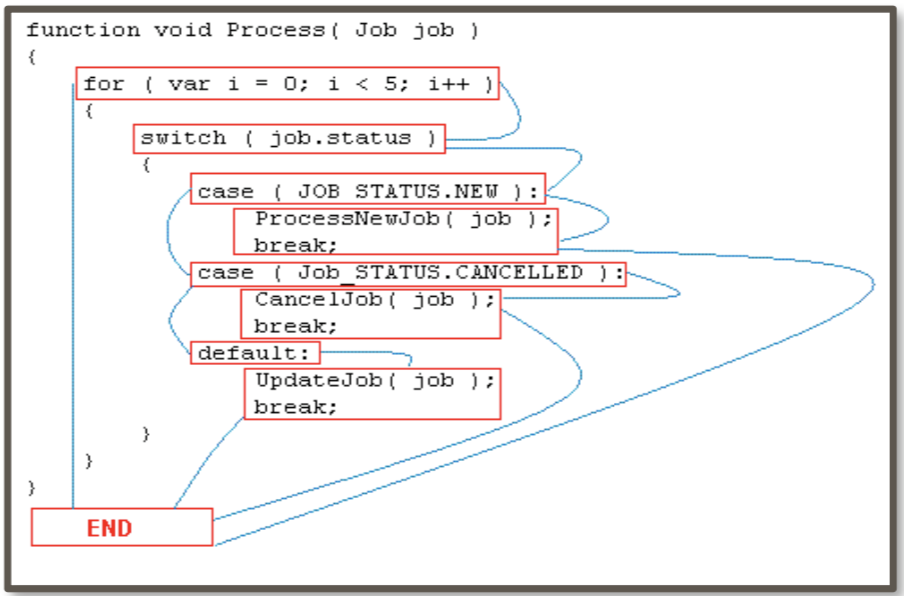
\includegraphics[scale=0.5]{assets/caclomatic_complexity.png} \\
		\textbf{Ablauf zu zyklischen Komplexität}
	\end{center}
	
	
	\subsubsection{Decision Points}
	Typische Entscheidungspunkte sind:
	\begin{multicols}{2}
	\begin{itemize}
		\item if
		\item for
		\item while
		\item case
	\end{itemize}
	\end{multicols}
	Oft falsch gemacht:
	\begin{itemize}
		\item switch-Statement selbst ist kein Entscheidungspunkt, wohl aber jedes einzelne case- Statement. Denn erst bei den case-Statements steht die Bedingung, welche entscheidet, ob der nachfolgende Block ausgeführt wird.
		\item Else und default sind keine Entscheidungspunkte, die Entscheidung wird im if, bzw in allen anderen case-Statements getroffen. Else und default sind dann nur noch die übrigbleibende Alternative.
		\item break: springt zwar auch im Kontrollfluss über folgende Statements hinweg, ist aber kein Entscheidungspunkt, da der Sprung unbedingt ist.
	\end{itemize}
	
	%Neues Kapitel, neue Seite
	\newpage
	
	
	\section{Logging}
	
    \section{Codebeispiele} \label{sec:codebeispiele}

    \subsection{RentalTest} \label{subsec:rentaltest}
    \lstinputlisting[language=Java]{assets/RentalTest.java}
    %Neues Kapitel, neue Seite
	\newpage
	

    \subsection{Checkstyle} \label{subsec:heckstyle}
    \lstinputlisting[language=XML]{assets/swc_checkstyle.xml}

    % Inhalt Ende
\end{document} 









